\documentclass{article}
\usepackage{xr}
\usepackage{lscape}

\usepackage{graphicx}
\usepackage{authblk}
\usepackage{amsfonts}
\usepackage{pifont}

\renewcommand{\tablename}{Supplementary Table}
\renewcommand{\figurename}{Supplementary Figure}
\newcommand{\rowgroup}[1]{\hspace{-1em}#1}


\begin{document}


\title{Eagle: Making multiple-locus association mapping on a genome-wide scale routine}
\author[1]{Andrew W. George}
\author[1]{Arunas Verbyla}
\author[2]{Joshua Bowden}

\affil[1]{Data61, CSIRO, Australia.}
\affil[2]{IM \&T, CSIRO, Australia.}

\maketitle






\begin{landscape}

\begin{table}
\caption{{\bf Implementation and methodology attributes of eight computer programs/packages for genome-wide association mapping.} For the different types of model, 
LMM is linear mixed model.  GLM is generalised linear model., GLMM is generalised linear mixed model, and RF is random forests. 
}
\label{suptabsummary}
\vspace{0.5cm}
\begin{tabular}{lcccccccc} \hline
                                                   Attributes                  & {\bf Eagle}                                 & {\bf bigRR}             & {\bf glmnet}            & {\bf LMM-Lasso}                    & {\bf MLMM} & {\bf r2VIM}      & {\bf FaST-LMM} & {\bf GEMMA} \\  \hline
{\em Implementation}    &         &            &             &                   &            &                &      &      \\ 
\hspace{1mm}  Purpose built$^a$    &   Yes     &    Yes      &  No   &   Yes  &  Yes  &  Yes  & Yes  & Yes          \\ [0.35cm]


\hspace{1mm}  Language                 &  R/C++       &    R        &      R       &     Python     &  R          &    R         &  C++ and     &   C++   \\  
                                                          &         &            &             &                   &            &                                     &   Python$^b$       &      \\  [0.35cm]

\hspace{1mm} GUI                            & Yes &    No      & No          &  No    &  No    &   No     & No     & No    \\  [0.35cm]




\hspace{1mm} Documentation        &  Videos,                &    R help       &  Vignettes,    &   Readme.txt,       &   Vignette,          &     R help           &   Videos,              &  User-manual,     \\  
                                                        &   user-manuals,    &                      &  R help         &    test script           &  R help              &                           &    user-manuals,  &   website  \\
                                                        &   website,    R help          &                      &                     &                              &                           &                           &    website            &    \\   [0.35cm]

                                                                         
\hspace{1mm} Additional fixed        &   Yes   &      Yes      &     Yes    &  No                 &      Yes      &      Yes          &      Yes & Yes     \\  
\hspace{1mm} effects$^c$               &           &                   &                 &                   &                   &                     &              &   adsf    \\  [0.35cm]

\hspace{1mm} Types of  &  Cont.      &   Cont.,          &   Cont.,           &   Cont.                 &   Cont.          &     Cont.           &   Cont.   &  Cont.    \\  
\hspace{1mm} trait data  &                &    binary,      &      binary,         &                   &            &                &      &      \\  
                                      &                &   count         &       count          &                   &            &                &      &      \\  [0.35cm]


\hspace{1mm} Data larger                   &   Yes    &      No      & No          &  No    &  No    &   No     & Yes      & No    \\  
\hspace{1mm} than memory                                             &         &            &             &                   &            &                &      &      \\  [0.8cm]


{\em Methodology}    &         &            &             &                   &            &                &      &      \\  
\hspace{1mm}  Model                     & LMM   &   &  GLMM &   GLM  & LMM  & RF & LMM   & LMM \\ [0.15cm]

\hspace{1mm} SNPs fitted       &    All/multiple      &    All       &   All        &      All          &  Multiple          &  Multiple              &   Single   &  Single   \\  [0.35cm]


\hspace{1mm}  Selection type              & Model   & Variable  &  Variable &  Variable  &  Model  &  Variable & Variable  & Variable \\  [0.35cm]

\hspace{1mm} Threshold free$^5$        &    Yes     &  No    &  No         &    No               &     Yes       &  No              &  No   & No      \\  [0.15cm]  \hline
           

\end{tabular}
{$^a$ \scriptsize{Specifically created for the analysis of GWAS data.}}\\
{$^b$ \scriptsize{Separate programs, one written in Python, the other C++}} \\
{$^c$ \scriptsize{Capacity for additional fixed effects (such as  age, sex, and/or population structure effects) to be included directly in the model.}} \\
\end{table}


\end{landscape}







\begin{landscape}

\begin{table}
\caption{Some of the key features possessed by Eagle and the other seven computer programs/packages for association mapping}
\label{suptabsummary}

\begin{tabular}{lccccccccc} 
                                &  \multicolumn{9}{c}{Computer Programs/Packages for Association Mapping} \\ \cline{2-10}
                                 & \multicolumn{6}{c}{Multiple-locus}  & & \multicolumn{2}{c}{Single-locus} \\  \cline{2-7}   \cline{9-10}
 Features                 & Eagle  & bigRR & glmnet & LMM-Lasso & MLMM & r2VIM     & & FaST-LMM & GEMMA \\  \hline
Purpose built$^1$    &   Yes     &    Yes      &  No   &  Yes  &  Yes  &  Yes && Yes & Yes           \\ [0.2cm]
Well documented$^2$           & Yes &   No   & Yes   & No     &   Yes     & No          && Yes    &    Yes    \\  [0.2cm]
Simultaneous   &    Yes     &    Yes        &   Yes          &      Yes             &  No          &  No              &&   No   &  No     \\  
fitting of SNPs     &         &            &             &                   &            &                &&      &      \\  [0.2cm]
Additional fixed effects$^3$          &   Yes   &      Yes      &     Yes    &  No                 &      Yes      &      Yes          &&      Yes & Yes     \\   [0.2cm]
Data larger than RAM$^4$                   &   Yes    &      No      & No          &  No    &  No    &   No     && Yes      & No    \\  [0.2cm]
Threshold free$^5$        &    Yes     &  No    &  No         &    No               &     Yes       &  No              &&  No   & No      \\  [0.2cm]
Informative error checking           &  Yes      &     No        &      No     &           No        &      No       &         No       && Yes  & No \\ \hline

\end{tabular}
{$^1$ \scriptsize{Specifically created for the analysis of GWAS data.}}\\
{$^2$ \scriptsize{More than just a readme file or comments in an example file. Programs/packages with a tick had a detailed user manual.}}\\
{$^3$ \scriptsize{Ability to handle additional fixed effects such as  age, sex, and/or population structure effects.}} \\
{$^4$ \scriptsize{Able to deal with data larger than the memory capacity of the computer.}} \\
{$^5$ \scriptsize{Results reported as the set of SNP closest to the genes influencing a trait. No need to construct thresholds to determine 
significance of the findings.}}\\
{$^6$  \scriptsize{All the programs terminated on errors. However, not all the programs informed the user of the cause and how to fix the errors.}}\\
\end{table}


\end{landscape}




\begin{figure}
\caption{Memory usage (in gigabytes) of Eagle and the other association mapping programs across 
the six simulation scenarios. The maximum amount of memory on the computer is 128 gigabytes. 
The x-axis is on the log scale. GEMMA, a single-locus implementation, had the lowest memory usage. 
Of the multiple-locus implementations, Eagle had the lowest memory usage. Also, it 
was the only multiple-locus 
implementation able to produce results for data under  scenario 10000 x 1.5M. This is due to its ability 
to handle data larger than the available memory of a computer. FaST-LMM was run where all the SNP data are used 
to estimate the relationship matrix (FaST-LMM$^{all}$)   and where genotype data from every five-hundredth SNP are used to 
estimate the relationship matrix (FaST-LMM$^{few}$)}.
\label{supfigmem}

\begin{center}
\includegraphics[width=15cm, height=15cm]{mem.eps}
\end{center}
\end{figure}



\begin{figure}
\caption{Power verse false discovery rates for Eagle and the single-locus methods GEMMA and FaST-LMM. 
FaST-LMM was run where all the SNP data are used 
to estimate the relationship matrix (FaST-LMM$^{all}$)   and where genotype data from every five-hundredth SNP are used to 
estimate the relationship matrix (FaST-LMM$^{few}$). Eagle has substantially higher power than the single-locus methods.   }


\label{supfigpowersingle}
\begin{center}
\includegraphics[width=15cm, height=15cm]{power2main.eps}
\end{center}

\end{figure}



\begin{table}
\caption{The median run times (in minutes) of Eagle and the other association mapping programs across the six simulation scenarios. }
\begin{tabular}{llcccccc}
              &           &  \multicolumn{6}{c}{Simulation Scenarios} \\ \cline{3-8}
 Method & Name & 150 x 5K & 1500 x 50K & 350 x 400K & 2000 x 500K & 4000 x 1.5M & 10000 x 1.5M \\ \hline
  Multiple & Eagle 	&	   0.08  &   1.62   &  \bf{2.7}1  &   \bf{13.65}   & \bf{127.63}  &   699.55  \\
               & MLMM 	&	   0.15    &  2.91    & 19.04  &  143.01  &  870.84  &     \\
               & glmnet 	&	  0.11     & 3.95    & 14.06    & 74.03    &        &    \\
               & r2VIM 	&	   0.09    &  3.66    &  5.51    & 50.59    & 380.52  &   \\ 
               & bigRR 	&	    1.01   & 113.35   &  54.99   & 1030.61  &        &     \\
               & LMM-Lasso 	&     0.57  &   52.08 &    92.20  & 1031.85 &           &     \\ \\
Single     &  GEMMA 	&      0.02  &   5.02   &   6.17  &   84.83   & 723.33  & 4071.60 \\
               & FaST-LMM$^{few}$ 	&    \bf{0.01}   &  \bf{0.80}   &   7.07   &  20.16   & 193.90   & \bf{346.19} \\ 
               & FaST-LMM$^{all}$   	&   0.03   & 2.96  &    7.90   &  41.27  &            &   \\ \hline
\end{tabular}

\end{table}


\end{document}
